\documentclass[tikz,border=10pt]{standalone}
\usetikzlibrary{calc}

\begin{document}
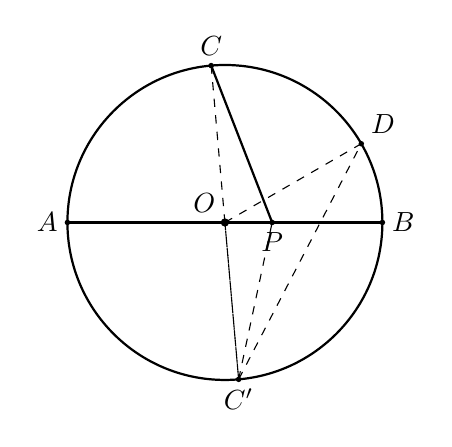
\begin{tikzpicture}
    % --- 定义全局参数 ---
    \def\R{2} % 圆的半径
    
    % --- 绘制圆 ---
    \draw[thick] (0,0) circle (\R);
    
    % --- 定义坐标 ---
    \coordinate (O) at (0,0);
    \coordinate (A) at (-\R,0);
    \coordinate (B) at (\R,0);
    \coordinate (C) at (95:\R); % C点位置
    \coordinate (Cp) at (95:-\R); % C'点位置，关于原点对称
    \coordinate (P) at (0.6,0); % P点位置，在AB上
    \coordinate (D) at (30:\R); % D点位置
    
    % --- 绘制点 ---
    \fill (O) circle (1.5pt) node[above left] {$O$};
    \fill (A) circle (1pt) node[left] {$A$};
    \fill (B) circle (1pt) node[right] {$B$};
    \fill (C) circle (1pt) node[above] {$C$};
    \fill (Cp) circle (1pt) node[below] {$C'$};
    \fill (P) circle (1pt) node[below] {$P$};
    \fill (D) circle (1pt) node[above right] {$D$};
    
    % --- 绘制连线 ---
    \draw[thick] (A) -- (B); 
    \draw[thick] (C) -- (P);
    
    % --- 绘制虚线 ---
    \draw[dashed] (C) -- (Cp);
    \draw[dashed] (Cp) -- (O);
    \draw[dashed] (Cp) -- (P);
    \draw[dashed] (Cp) -- (D);
    \draw[dashed] (O) -- (D);

\end{tikzpicture}
\end{document}